
    \begin{abstract_online}{Mechanism of Hydroxide Ion Transfer through Anion Exchange Membrane in Anion Exchange Membrane Fuel Cell: Investigation using Molecular Dynamics Simulation}{%
        \underline{V. Dubey}, A. Maity, S. Daschakraborty}{%
        }{%
        Department of Chemistry, IIT Patna, India}
    Anion exchange membrane fuel cells (AEMFCs) have great potential over proton exchange  membrane fuel cells (PEMFCs) due to cost-effective energy conversion. However, $OH^{-}$ ion  transport is a key obstacle. It is evident that $OH^{-1}$ ion can move through the hydrated AEM via  two ways: (i) Grotthuss mechanism either via water chain or via AEM membrane surface sites,  and (ii) Vehicular diffusion via Brownian motion. A recent study based on multistate empirical  valence bond (MS-EVB) by Chen et al. has proposed that the vehicular diffusion contributes  approximately $80 \%$ to the total diffusion of the hydroxide ion via the hydrated poly-vinyl  benzyltrimethylammonium (PVBTMA) polymer. The remaining $20 \%$ is contributed by the  Grotthuss mechanism. This striking importance on vehicular diffusion motivated us to focus on  the vehicular diffusion of the hydroxide ions. In addition, a couple of more recent studies have  demonstrated a much larger importance of Grotthuss diffusion over the vehicular diffusion of  hydroxide ion in a different AEM. Thus there is a need for more investigation to understand the  $OH^{-1}$ ion transport. In this work, we used empirical force-field based classical MD simulation to  understand the structure and vehicular diffusion of $OH^{-1}$ ion. However, this method is inadequate  to explain reactions or transformations where bond breaking and formation occurs. But the  vehicular diffusion is obtained here in a straightforward way. This gives us a better  understanding of the possible role of $OH^{-1}$ ion transport via vehicular diffusion; results will be  discussed in the poster in more detail.  \begin{center}  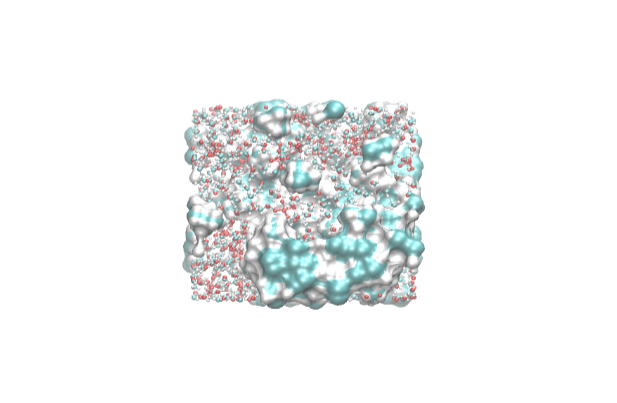
\includegraphics[width=0.65\linewidth]{abstracts/txt/figures/vikas-dubey.png}  \end{center}  
    
        \textbf{References} \newline{}[1] Chen, C.; Tse, Y. L. S.; Lindberg, G. E.; Knight, C.; Voth, G. A., J. Am. Chem. Soc. 2016, 138,\newline{}991−1000.\newline{}[2] Dong, D.; Zhang, W.; Duin, A. C. T. van; Bedrov, D., J. Phys. Chem. Lett. 2018, 9, 825-829.
    \end{abstract_online}
    